\documentclass[12pt,twoside]{report}   % or 11 pt if you're desperate for space.
\usepackage{amsmath, amssymb, amsthm, pgf, tikz}
\usepackage{graphicx, microtype, hyperref}
\usetikzlibrary{arrows,automata}
\usepackage{fancyhdr}
\usepackage[toc,page]{appendix}
\usepackage{caption}
\usepackage{subcaption}
\usepackage{float}
\usepackage{parskip}
\usepackage{listings}
\usepackage[utf8]{inputenc}
\usepackage{color}
\usepackage{tcolorbox}
\definecolor{codeblue}{rgb}{0.12, 0.56, 1.0}
\definecolor{codegreen}{rgb}{0.3,0.73,0.09}
\definecolor{codegray}{rgb}{0.5,0.5,0.5}
\definecolor{codeorange}{rgb}{0.93, 0.53, 0.18}
\definecolor{codewhite}{rgb}{0.97, 0.97, 1.0}
\definecolor{backcolour}{rgb}{0.15, 0.15, 0.15}
\lstdefinestyle{mystyle}{
    backgroundcolor=\color{backcolour},   
    commentstyle=\color{codegreen},
    keywordstyle=\color{codeblue},
    numberstyle=\tiny\color{codegray},
    stringstyle=\color{codeorange},
    basicstyle=\small\color{codewhite},
    breakatwhitespace=false,         
    breaklines=true,                 
    captionpos=b,                    
    keepspaces=true,                 
    numbers=left,                    
    numbersep=5pt,                  
    showspaces=false,                
    showstringspaces=false,
    showtabs=false,                  
    tabsize=2
}

\hypersetup{
    colorlinks=true,
    citecolor=red,
    linkcolor=blue,
    filecolor=blue,      
    urlcolor=blue,
}
 
\lstset{style=mystyle}
\def\ContinueLineNumber{\lstset{firstnumber=last}}
\def\StartLineAt#1{\lstset{firstnumber=#1}}
\let\numberLineAt\StartLineAt
%%%%%%%%%%%%%%%%%%%%%%%%%%%%%
\newcommand{\bkt}[1]{\left( #1 \right)}
\newcommand\aap{}

\newtheorem{theorem}{Theorem}[section]
\newtheorem{maintheorem}[theorem]{Main Theorem}
\newtheorem{definition}[theorem]{Definition}
\newtheorem{lemma}[theorem]{Lemma}
\newtheorem{proposition}[theorem]{Proposition}
\newtheorem{corollary}[theorem]{Corollary}


%%%%%%%%%%%%%%%%%%%%%%%
% This stuff below sets the page layout. Don't change these.
\addtolength{\topmargin}{-2.7cm}
\addtolength{\textheight}{5cm}
\setlength{\headheight}{15pt}
\evensidemargin 14pt
\oddsidemargin 14pt
\textwidth 6.2in
\raggedbottom
\widowpenalty=5000
\clubpenalty=1000

%%%%%%%%%%%%%%%%%%%%%%%

\begin{document}


\begin{titlepage}
    \begin{center}
        \vspace*{1cm}
        
        \Huge
        \textbf{Using Mathematics with Python}
        
        \vspace{0.5cm}
        \LARGE
        Student Number 201503311
        
        \vspace{1.5cm}
        
        \textbf{Michael G. Turner}
        
        \vfill
        
        A thesis presented for the degree of\\
        Masters in Mathematics
        
        \vspace{0.8cm}
        
        \includegraphics[width=0.4\textwidth]{HullShield.pdf}
        
        \Large
        School of Mathematics and Physical Sciences\\
        University of Hull\\
        United Kingdom\\
        $30^{\text{th}}$ April 2018
        
    \end{center}
\end{titlepage}

\thispagestyle{plain}
\begin{center}
    \Large
    \textbf{Using Mathematics with Python}
    
    \vspace{0.4cm}
    \large
    Student Number 201503311
    
    \vspace{0.4cm}
    \textbf{Michael G. Turner}
    
    \vspace{0.9cm}
    \textbf{Abstract}
\end{center}

With the rapid increase in computational technologies, computers are becoming more able to perform complex mathematical calculations and the worlds dependencies on computers is continuing to grow. Today, having the skills to read and write in a programming language is the highest in demand. So much, in fact, that it is becoming a basic requirement with the introduction of learning how to code being implemented in schools. Python is one of the easiest to learn from scratch. It is the tool that can take the mathematics of Bayesian analysis and perform various forms of data analysis on a given data set like calculating the trace, mean, standard deviation, plotting the results, all while the mathematics happens on the inside.

The main aims of this report are to give details into what mathematics are being used behind the scenes in Python. To understand the methods for setting up an accurate model for our data analysis, how our model is passed into Python and to present the results to see what conclusions our analysis draws, whether it is proving global warming exists or that a percentage of our universe is Dark Matter.

\tableofcontents

\chapter*{Introduction}\thispagestyle{plain}

Though Python is regarded as one of the more easier programming languages to learn, it still requires time to understand the basics. After gradually progressing, becoming more familiar with the way problems can be approached, I began looking into the different uses that Python can have. After considering different tasks to take on I decided to investigate how to solve an ODE with numerical methods for my first semester of third year. The most stimulating of these was with an ODE that cannot be solved analytically. Thinking back to mathematics of the past, this would mean that there are physical problems that cannot be modelled. But, using a numerical approach with Python, the solution can be calculated and plotted, giving us the power to model complex situations with ease that was never possible before. An example is the following ODE which governs an oscillating spring mass
\begin{align*}
mu^{\prime\prime} + \beta u^{\prime} + ku = F(t) = \sin(t^2),\,\,u(0) = 0,\,\,u^{\prime}(0) = -1
\end{align*}

\begin{figure}[H]
\centering
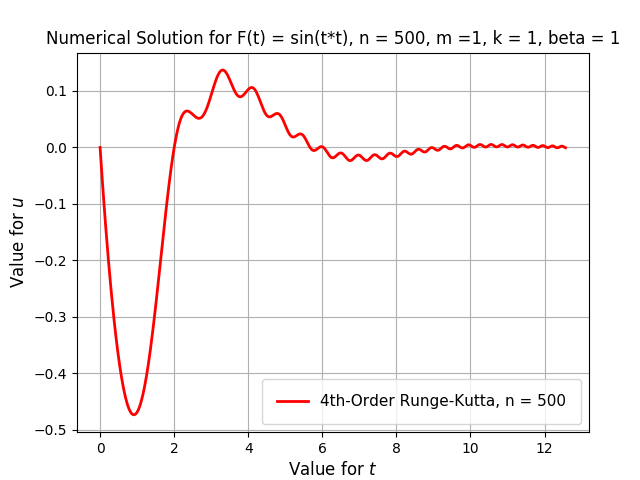
\includegraphics[width = 5in]{Kuttaadv.png}
\caption{Solution for $\mu^{\prime\prime} + \beta u^{\prime} + ku = \sin(t^2)$}
\label{figKuttaadv}
\end{figure}

\pagebreak
Once the first semester had come to a close, there was the decision of what to look into next? I concluded on studying the main process of Python. Data analysis is the biggest use for Python and is what I have been studying for all of second semester, which is the main focus of my thesis. It will cover the core approach to take when performing data handling. How to take in data and make sense of it, which is a valued skill on a CV.

I also wanted to focused on using a Bayesian analysis approach. I am a very thought orientated individual. Before I make a decision, I am considering the possible outcomes of each decision. This is what draws me to a Bayesian view on probability so naturally. But it is still a daunting thing to understand at first, but with the application of Python it becomes much more clear.

Python is the most important programming language for data analysis because of its huge advantages like amazing visual packages and a vast collection of data science libraries like Pandas, NumPY, Scipy and PyMC, all of which we will use throughout. It has an astounding ability to take difficult tasks like producing probability density functions of any given parameter in a statistical model and making it into a few lines of code. I did not know any Python from the start of the academic year and now I am able to present an entire thesis for why it is such an important tool in modern data statistics. If you would like to view and download the different Python codes used in my thesis then feel to visit my public GitHub repository at \url{https://github.com/iMikeT/MathProject}. Now, without further ado, we shall begin.

\newpage
\pagestyle{fancy}
\renewcommand{\chaptermark}[1]{ \markboth{#1}{} }
\renewcommand{\sectionmark}[1]{ \markright{#1}{} }
\fancyfoot{}
\fancyhead[RO,LE]{\thepage}
\fancyhead[LO]{\thesection\,\,\rightmark}
\fancyhead[RE]{\thechapter\,\,\leftmark}
\chapter{Bayes' Theorem}\label{Bayes' Theorem}

Before I dive deep into the main aspects discussed in the introduction, there are two fundamental differences in how I can view probability. One is the \textbf{Frequentist} approach and the other is the \textbf{Bayesian} approach. The best way to understand the differences is with a little example.

\section{Flipping a Coin}\label{Flipping a Coin}

\subsection{The Frequentist}\label{The Frequentist}

With the Frequentist view, we can think about probability of flipping a head, $P(h)$, as being the \textit{relative frequency} of getting a head in an infinitively long series of \textit{identical} flips. This can be represented in a mathematical expression as
$$P(h) = \lim_{n\to\infty} \frac{h}{n}$$
Here $h$ is the number of heads and $n$ is the total number of trials. There are some important assumptions being made in the Frequentist view. One that the data can vary, but the other is that the parameters are fixed. What are the parameters? Well, it comes from that sneaky term \textit{identical}.

Suppose that I flipped the coin at $67.3$cm from the ground and that the coin had an orientation to the ground that was an angle of $32^{\circ}$ relative to the horizontal and $2^{\circ}$ relative to the vertical and I repeated this set up \textit{exactly} then I should expect to get a certain value out with every flip because the system is in itself deterministic, right? This is where we encounter issues with the Frequentist view with what is truly meant by the term identical. We could possibly determine the coin to be a set height from the ground but allow the orientation to alter, but then we start to enter a subjective view for what identical means which goes against the Frequentist belief. For a real life scenario like this there is always going to be a sense of uncertainty because the experiment cannot be recreated exactly as before. This is something that is involved with Bayesian analysis.

\subsection{The Bayesian}\label{The Bayesian}

With the \textbf{Bayesian} view, we think of probability of flipping a head as the number of heads divided by the number of possible outcomes, which are all to be \textit{equally} likely. What this means is that we could quantify all the possible orientations of the coin, which will be our \text{initial} conditions, and then look at the forces acting on the coin. We can then combine these and then think about for each of these conditions, what value will the coin give? So the number of possibilities is given by the number of initial conditions and the number of heads represents the total number of heads we get across all these different possibilities.

The assumptions being made this time are that the data is fixed. What that would mean is that, given some initial condition like the orientation and height of the coin, we would get the same value every time. But the reason we do not is because the parameters can vary. So the Bayesian probability does not represent a long run frequency of getting a head but rather an uncertainty in that we do not know exactly what the initial orientation of the coin we are left with some underlying uncertainty with whether we will get a head or a tails.

This approach seems a lot more related to the real world as it is almost common sense to know that you can never be \textit{completely} certain if you will get a heads or a tails. And it is also important that the Bayesian view does not rely on an infinite number of samples. It is okay with this example as theoretically you could flip a coin an infinite number of times, there are some cases where this is not favourable.

\section{Conditional Probability}\label{Conditional Probability}

Conditional probability of, say an event $B$, is the probability an event $B$ will occur given we have knowledge of another event $A$ that has already passed. This is written as $P(B\mid A)$. If the two events are \textbf{independent} of each other then the probability of event $B$ occurring given event $A$ is simply just the probability of event B occurring, written as $P(B)$.

Bayes' Theorem describes how to update a probability given evidence. It is as follows.
\vspace{5pt}
\begin{theorem}
Given an parameter $a$ and data $b$, the relationship between the probability of $a$ before the data, $P(a)$, and the probability of $a$ given the data, $P(a\mid b)$, is given by
\end{theorem}
\begin{align}\label{Bayes' Formula}
\overbrace{P(a\mid b)}^\text{posterior} = \frac{\overbrace{P(b\mid a)}^\text{likelihood}}{\underbrace{P(b)}_\text{evidence}} \overbrace{P(a)}^\text{prior}
\end{align}
(See \cite{1} for a review)

Now there is a slight technicality here, we have to bring in the \textit{prior} to perform our analysis. This represents our \textit{``assumption''} for the value of $A$ before viewing the value $B$. The prior is therefore frowned upon by the frequentist because there is the arguable idea that it brings in subjectivity into the strict manner of probability. But, then again, a prior can be just another assumption made while modelling the situation. Which would then make it just as objective as any of the other assumptions made in the frequentist model. I think that this is very true. A prior is an assumption related to what I assume the probability to be distributed as. If it was rainy yesterday I can assume the probability that it will be sunny tomorrow increases because the days are not independent. It has to stop raining at some point because the clouds will not reset over night to have the same amount of water. The resource is not unlimited just like everything in nature.

\subsection{The Prior, Likelihood and Posterior}\label{The Prior, Likelihood and Posterior}

\begin{itemize}
\item The \textbf{prior} is what reflects the information that we know about the value of some parameter before viewing the data $B$. If nothing is known about the parameter then we use a \textbf{flat prior} which does not expose much information.
\item The \textbf{likelihood} is our way of introducing the data to the process. It represents how \textit{plausible} the data is observed given a set of parameters.
\item The \textbf{posterior} is a probability distribution of the parameters in our model given the data. It is what we know about the problem and relates to the prior and the likelihood. If the prior and likelihood are both vague then we will get a posterior that reflects these vague beliefs. It can be thought of as the updated version of the prior with the given data.
\end{itemize}

The \textbf{evidence} is the probability of getting the data averaged over all possible values. It can be thought of simply as a \textbf{normalising factor} and will not be an issue if we neglect because we are not concerned about the true values of the parameters. Thus, we can rewrite Bayes' theorem as a proportionality (A more general form than our example before)
\begin{align}\label{Bayes' Formula Proportional}
P(A\mid B) \propto P(B\mid A)P(A)
\end{align}
Where $A$ is the \textit{hypothesis} and $B$ is the \textit{data}. To gather a true understanding for what each role actually \textit{does}, it will be beneficial to do a simple example.

\section{Simple Example}\label{Flip of a Coin}

We can continue with our coin flipping example used in \S\ref{Flipping a Coin} and start to work with the methods by placing in some values. We toss a coin $n$ times and record the number of heads $h$ and tails $t$. Using just this simple data we can deduce answers to possible questions about the problem like \textit{``Is the coin fair?''}. So, to do this, we will need our data, which is assumed we have already collected, and a model. 

\subsection{The Model}\label{The Model}

Let us set up an understanding for how the bias can be for this problem. A coin a bias of $1$ will always land on heads. A coin with a bias of $0$ will always land on tails. A coin with a bias of $0.5$ will land on heads and tails evenly. We will use the parameter $\theta$ for the bias. Then, by Bayes' theorem, we have
\begin{align}\label{Bayes' Theorem Proportional Coin}
P(\theta\mid h) \propto P(h\mid \theta)P(\theta)
\end{align}
Now, we need to choose which prior and likelihood we should use.

\subsubsection{Choosing the Likelihood}\label{Choosing the Likelihood}

Firstly, let us assume that each coin toss is independent of each other. And that only heads
or tails in a possible outcome (no side shots). We know that there are a fixed number of flips and the probability of getting a heads is constant throughout. These are all traits associated with a binomial experiment so the likelihood is the \textbf{binomial distribution} which has a probability mass function (pmf)
\begin{align}\label{Binomial Distribution}
P(h\mid\theta) = \frac{n!}{h!(n - h)!}\theta^h(1 - \theta)^{(n-h)}
\end{align}
This gives us the probability of getting exactly $h$ heads out of $n$ flips. An interesting observation is that, if we consider the bias extremes and set $\theta = 1$, this gives the result $P(h\mid\theta) = 0$. This is down to the fact that this coin doesn't exist. The \textit{coin} would have only one side which breaks the binomial condition that there are two possible outcomes. This is more of a ball than a coin now. But the measure of bias is still valid as $\theta \in (0,1)$.

\subsubsection{Choosing the Prior}\label{Choosing the Prior}

One choice for the prior is the \textbf{beta distribution}. This distribution is good for our parameter $\theta$ because it is restricted between $0$ and $1$. The first term normalises the distribution so that it will always integrate to $1$. It has two parameters, $\alpha$ and $\beta$, that control the distribution. The pmf is given by
\begin{align}\label{Beta Distribution}
P(\theta) = \frac{\Gamma\big(\alpha + \beta\big)}{\Gamma\big(\alpha\big)\Gamma\big(\beta\big)}\theta^{\alpha - 1}\big(1 - \theta\big)^{\beta - 1}
\end{align}
This distribution is something called a \textbf{conjugate prior} to the binomial distribution. This means that we will get a beta distribution as a posterior. This makes the posterior easier to solve analytically. It is an older practice and now, because of numerical methods, this is not as much of an issue. Python can perform the difficult calculations. But it will make the mathematics easier for the moment.

\subsubsection{Getting the Posterior}\label{Getting the Posterior}

This is where we start cooking! (mathematically, of course) Recall equation (\ref{Bayes' Theorem Proportional Coin}) that says the posterior is proportional to the likelihood multiplied by the prior. So, by using equations (\ref{Binomial Distribution}) and (\ref{Beta Distribution}) we get the following
\begin{align*}
P(\theta\mid h) &\propto \bigg(\overbrace{\frac{n!}{h!(n - h)!}\theta^h(1 - \theta)^{(n-h)}}^\text{Likelihood}\bigg)\bigg(\overbrace{\frac{\Gamma\big(\alpha + \beta\big)}{\Gamma\big(\alpha\big)\Gamma\big(\beta\big)}\theta^{\alpha - 1}\big(1 - \theta\big)^{\beta - 1}}^\text{Prior}\bigg)\\
&\propto \Big(\theta^h(1 - \theta)^{(n-h)}\Big)\Big(\theta^{\alpha - 1}\big(1 - \theta\big)^{\beta - 1}\Big)\\
&\propto \theta^{(\alpha - 1) + h}\big(1 - \theta\big)^{(\beta - 1) + (n - h)}
\end{align*}
There is a relation between this form and the form of the beta distribution as
\begin{align*}
\alpha_\text{posterior} = \alpha_\text{prior} + h,\quad\beta_\text{posterior} = \beta_\text{prior} + (n - h)
\end{align*}
This means that the posterior is the following beta distribution
\begin{align*}
P(\theta\mid h) = \text{Beta}\big(\alpha_\text{prior} + h,\,\beta_\text{prior} + (n - h)\big)
\end{align*}

\subsection{Computing the Posterior}\label{Computing the Posterior}

Using the above analytic expression, we can compute the final result using Python. For example, let us set the number of flips $n = 50$ and the number of times we get heads $h = 18$. The prior is set to follow the belief that the coin is fair. So, we believe that over 50 experiments, we will get $h=25$ and $t=25$. Then our prior is $\text{Beta}(25,25)$. Now, in our experiment, we have that over 50 experiments, we received $h=18$ and $t=32$. Then our posterior is $\text{Beta}(25+18,25+32) = \text{Beta}(43,57)$. We can then calculate and plot the results with Python.
\begin{figure}[H]
\centering
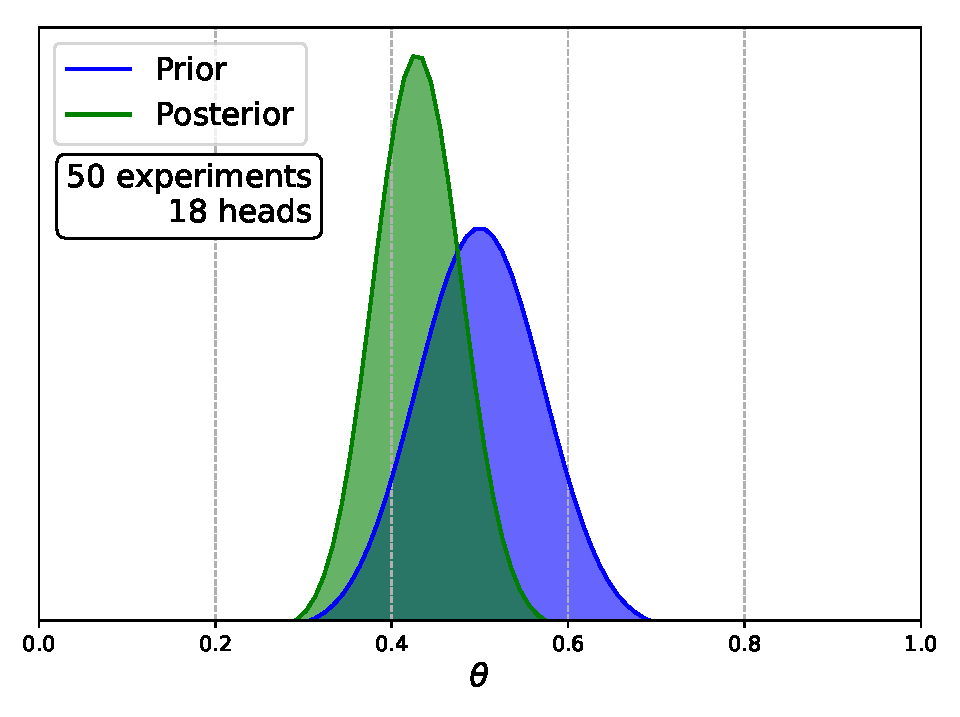
\includegraphics[width = 5in]{Final.pdf}
\caption{Plot of $p(\theta\mid h)$ with fair prior}
\label{figCoinFlipGood}
\end{figure}
\pagebreak
The posterior is moving towards the left which would suggest that the coin is not fair, as our prior had assumed, and that the bias $\theta < 0.5$. We could approximate the bias as being $\theta \approx 0.43$ using the peak of the posterior distribution. This implies that the coin has a sightly higher probability of landing on tails than heads with each flip. Doing this example is to show the importance of choosing a prior with knowledge of the given situation. And to outline this fact further, we can play through this again with a poor prior.

Say we choose the prior to be the belief that over 50 flips, we get 40 heads. Then our prior is Beta$(40,10)$. We shall keep the same data as $50$ flips and $18$ heads but this poor prior will result in our posterior being Beta$(58,42)$. Clearly this prior would never be considered if you are aware what a fair coin flip is. But consider someone that is not familiar with what a coin is at all and chooses this prior. Then it will result in the following figure.
\begin{figure}[H]
\centering
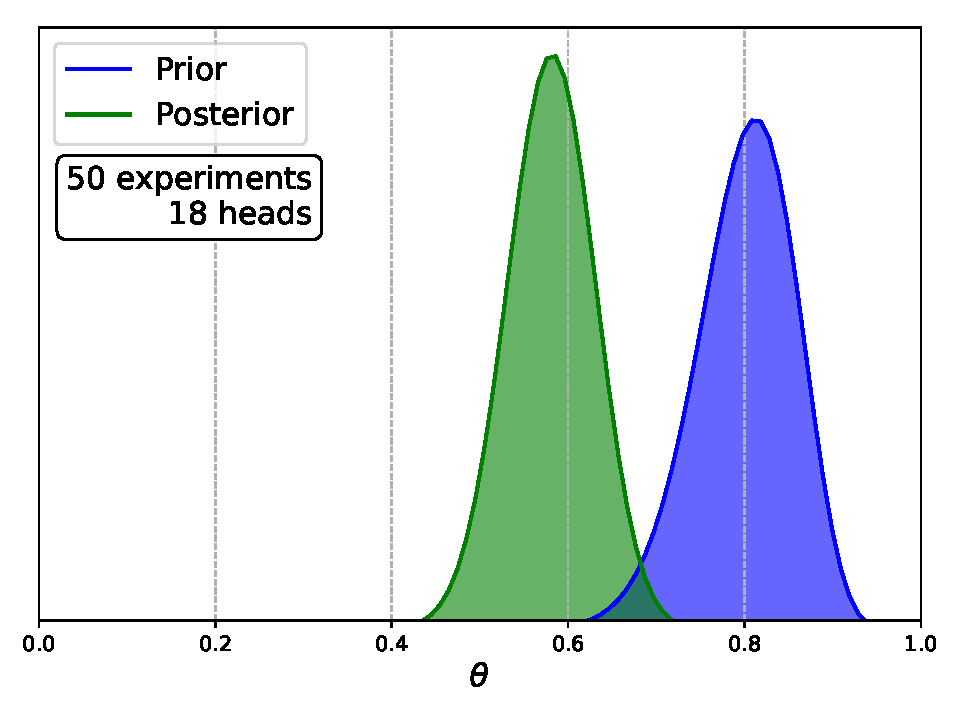
\includegraphics[width = 5in]{BadPrior1.pdf}
\caption{Plot of $p(\theta\mid h)$ with poor prior}
\label{figCoinFlipBad1}
\end{figure}

It is clear now what was suggested, that the bias would be $40/50 = 0.8$ just as the peak of the prior is very close to that value of $\theta$. The error in the prior then results in error with the posterior. It is giving us the estimate that the coin has a bias of $\theta \approx 0.56$ which does not reflect our data. This suggests our coin has a slightly higher probability of landing on heads. But the data shows we got 18 heads and 32 tails. This tells us that something is wrong. Another sign of an error is that the separation or difference between the two distributions is large. This could point out that the prior is off from the value of $\theta$. The only way to investigate these signs would be to alter the prior, as our data is fixed in the Bayesian view. So we could then adjust the prior to a \textit{new} belief that the bias of the coin is less than $0.8$ and repeat the process.

To reiterate, the posterior is our updated prior given the data. The figure \ref{figCoinFlipGood} gives us an understanding about Bayesian analysis such as:
\begin{itemize}
\item The result is a posterior distribution, not a number. It gives us a distribution on the probability with our data.
\item The most plausible value is the peak of the distribution as highlighted before.
\item The spread of the posterior distribution is proportional to the uncertainty of the value for $\theta$. The less spread, the more certain the value.
\item How quickly different posteriors converge to the same distribution depends on the data and the model.
\item The posterior we get from computing with 50 flips \textit{once} will be the same as if we computed the posterior 50 times with each one adding one extra observation and using the previous posterior as the new prior.
\end{itemize}
(See \cite{2} for more detail of \S\ref{Conditional Probability}, \S\ref{Flip of a Coin})

\chapter{Markov Chain Monte Carlo Algorithms}\label{MCMC}

Markov Chain Monte Carlo (MCMC) is a process for generating samples $x^{(i)}$ while \textit{wondering} the possible states $X = \{x_1,x_2,\ldots,x_n\}$ using the Markov chain mechanism which is constructed so that the samples $x^{(i)}$ replicate samples drawn from the target distribution $P(x)$. A Markov chain on a finite state space where $x^{(i)}$ can take any state $X$ is called a Markov chain if 
\begin{align}\label{Markov Chain Def}
P(x^{(i)}\mid x^{(i-1)},x^{(i-2)},\ldots,x^{(1)}) = P(x^{(i)}\mid x^{(i-1)})
\end{align}

The progression of the Markov chain in a state space $X$ depends only on the current state of the chain and a fixed \textbf{transition} matrix, denoted \textbf{P}. To gather a more intuitive understanding we should see an example.

\section{What's for dinner?}\label{What's for Dinner}

Consider a Markov chain with $3$ states ($n=3$). The corresponding transition matrix, illustrated by Figure \ref{figMarkovProcess}, represents the probabilities of what I am hungry for, given the food I had on the preceding day
\begin{align*}
\textbf{P} = \begin{bmatrix}
	& P & B & H \\
    P & 0.5 & 0.3 & 0.2 \\
    B & 0.25 & 0.5 & 0.25 \\
    H & 0.4 & 0.4 & 0.2
\end{bmatrix}
\end{align*}
This defines the probability of going from a state $x_i$ to $x_j$ where $i,j = 1,2,\ldots,n$. So the element $[\textbf{P}]_{ij}$ is the probability that a day with dinner $i$ will be followed by a day with dinner $j$ e.g. $[\textbf{P}]_{12}$ is a $30\%$ chance that a pizza will be followed by a burger.

\begin{figure}[H]
\centering
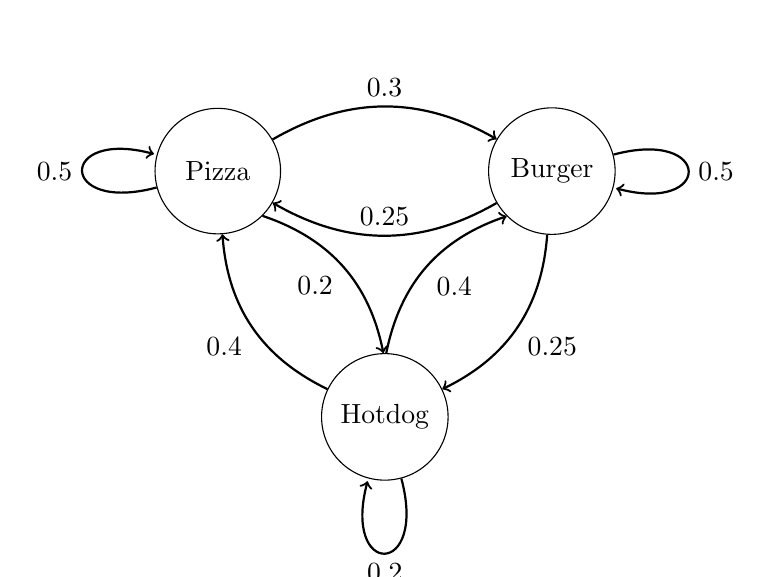
\begin{tikzpicture}[auto]
\tikzstyle{node} = [circle, draw,text width=4.5em, text badly centered, node distance=3cm, inner sep=0pt]
\node [node] (node0) {Hotdog};
\node [node,above left of=node0,yshift=1cm] (node1) {Pizza};
\node [node,above right of=node0,yshift=1cm] (node2) {Burger};
\path (node0) edge [bend left,->,thick] node [pos=0.5] { 0.4} (node1);
\path (node1.south east) edge [bend left,->,thick] node [pos=0.5,below left] { 0.2} (node0);
\path (node1) edge [bend left,->,thick] node [pos=0.5] { 0.3} (node2);
\path (node2) edge [bend left,->,thick] node [pos=0.5] { 0.25} (node0);
\path (node2) edge [bend left,->,thick] node [above,pos=0.5] {0.25} (node1);
\path (node2.south west) edge [bend right,<-,thick] node [pos=0.5,below right] {0.4} (node0);
\path (node0) edge [loop below,->,thick] node [pos=0.5] {0.2} (node0);
\path (node1) edge [loop left,->,thick] node [pos=0.5] {0.5} (node1);
\path (node2) edge [loop right,->,thick] node [pos=0.5] {0.5} (node2);
\end{tikzpicture}
\caption{Transition graph }
\label{figMarkovProcess}
\end{figure}

So, say I have pizza for dinner on day $1$. This is represented as the vector
\begin{align*}
{x}^{(1)} = [1,0,0]
\end{align*}

Now the dinner I will have on day $2$ is given by
\begin{align*}
{x}^{(2)} = {x}^{(1)}\textbf{P} = [1,0,0]\begin{bmatrix}
    0.5 & 0.3 & 0.2 \\
    0.25 & 0.5 & 0.25 \\
    0.4 & 0.4 & 0.2
\end{bmatrix} = [0.5,0.3,0.2]
\end{align*}

There is a $50\%$ chance I will have pizza again on day $2$.

The dinner for day $3$ is similar
\begin{align*}
{x}^{(3)} = {x}^{(2)}\textbf{P} = {x}^{(1)}\textbf{P}^2 = [1,0,0]\begin{bmatrix}
    0.405 & 0.38 & 0.215 \\
    0.35 & 0.425 & 0.245 \\
    0.38 & 0.4 & 0.22
\end{bmatrix} = [0.405,0.38,0.215]
\end{align*}

So the general formula for day $n$ is
\begin{align*}
{x}^{(n)} = {x}^{(1)}\textbf{P}^n
\end{align*}

As the days go on, the vector ${x}^{(n)}$ tends to what is called a \textbf{steady state} vector which represents the probability of what I will have for dinner on all days, with the assumption that this is all I will eat for the rest of my days, no matter what the initial meal (distribution) is. This is a very important piece of MCMC simulation. For any initial distribution, the Markov chain will converge to the invariant distribution $P(x)$, represented as
\begin{align}\label{Stationary Vector}
P(x) = P(x)\textbf{P}
\end{align}

Thus,
\begin{align*}
P(x)\textbf{P} = P(x) = P(x)\textbf{I}
\end{align*}
\vspace{-30pt}
\begin{align*}
\Rightarrow\quad P(x)(\textbf{P} - \textbf{I}) &= P(x)\left(\begin{bmatrix}
    0.5 & 0.3 & 0.2 \\
    0.25 & 0.5 & 0.25 \\
    0.4 & 0.4 & 0.2
\end{bmatrix} - \begin{bmatrix}
    1 & 0 & 0 \\
    0 & 1 & 0 \\
    0 & 0 & 1
\end{bmatrix}\right)\\
&= P(x)\begin{bmatrix}
    -0.5 & 0.3 & 0.2 \\
    0.25 & -0.5 & 0.25 \\
    0.4 & 0.4 & -0.8
\end{bmatrix} = \boldsymbol{0}\\
\end{align*}

Note the condition $P_1 + P_2 + P_3 = 1$. Using this we can solve these simultaneous equations to give us the steady state distribution
\begin{align*}
[P_1,P_2,P_3] = [0.3774,0.4025,0.2201]
\end{align*}

This means that, as the days go on, I will have pizza for $37.74\%$, burger for $40.25\%$ and hotdog for $22.01\%$ of days in the future. It is important to note that Equation (\ref{Stationary Vector}) only holds if the transition matrix \textbf{P} satisfies the following conditions:
\begin{itemize}
\item Irreducibility: For any state of the Markov chain, there is a positive probability of visiting
all other states. That is, the matrix T cannot be reduced to separate smaller matrices.
\item Aperiodicity: The chain should not get trapped in cycles.
\end{itemize}

A sufficient, but not necessary, condition to ensure that a particular $P(x)$ is the desired
invariant distribution is the following reversibility condition
\begin{align}\label{reversibility}
P\left(x^{(i)}\right)\textbf{P}\left(x^{(i-1)}\mid x^{(i)}\right) = P\left(x^{(i-1)}\right)\textbf{P}\left(x^{(i)}\mid x^{(i-1)}\right)
\end{align}

Summing both sides over $x^{(i-1)}$ gives
\begin{align*}
P\left(x^{(i)}\right) = \sum_{x^{(i-1)}}P\left(x^{(i-1)}\right)\textbf{P}\left(x^{(i)}\mid x^{(i-1)}\right)
\end{align*}
(See \cite{3} for more detail)

After taking in all of this you might be asking ``what does all of this mean for problems in Python?''

\section{MCMC Sampling}\label{MCMC Sampling}

MCMC samplers are aperiodic Markov chains that have the target distribution as the invariant distribution. They provide algorithms for sampling from a probability distribution by building a Markov chain, which satisfies the above conditions, that has the desired probability distribution as the \textbf{stationary distribution}. One of these algorithms is the \textbf{Metropolis-Hastings} algorithm.
\pagebreak
\subsection{Metropolis-Hastings algorithm}\label{Metropolis-Hastings algorithm}

By far the most popular MCMC method, the Metropolis-Hastings (MH) algorithm produces a Markov chain that converges to a given distribution that is its stationary distribution. The transition distribution $\textbf{P}(x\mid y)$ is the probability of transitioning into state $y$, given the current state is $x$. Finding $\textbf{P}(x\mid y)$ that satisfies the reversibility condition first requires an arbitrary ``switch'' distribution $\textbf{Q}(y\mid x)$. This is so we obtain $\textbf{P}(x\mid y)$ if the switch is accepted with acceptance probability $\textbf{A}(x\mid y)$.

If $y=x$ then the reversibility conditions holds. If $y\neq x$ then
\begin{align*}
\textbf{P}(y\mid x) = \textbf{Q}(y\mid x)\textbf{A}(x\mid y)
\end{align*}

Substituting this into the reversibility condition yields
\begin{align*}
P(y)\textbf{Q}(x\mid y)\textbf{A}(y\mid x) &= P(x)\textbf{Q}(y\mid x)\textbf{A}(x\mid y)\\
\Rightarrow\quad\frac{\textbf{A}(x\mid y)}{\textbf{A}(y\mid x)} &= \frac{P(y)\textbf{Q}(x\mid y)}{P(x)\textbf{Q}(y\mid x)}
\end{align*}

Note that the probability $A$ takes values $[0,1]$ so
\begin{align*}
\textbf{A}(x\mid y) = \min\left\{1, \frac{P(y)\textbf{Q}(x\mid y)}{P(x)\textbf{Q}(y\mid x)}\right\}
\end{align*}

Now, with these results, The MH algorithm works as follows:
\begin{enumerate}
\item Start at a random or educated guess for initial parameter $x^{(i)}$.
\item Choose a new parameter value $x^{(i+1)}$ sampling from a uniform\\ distribution $\textbf{Q}\left(x^{(i+1)}\mid x^{(i)}\right)$.
\item Calculate the probability of accepting $x^{(i+1)}$ by using the MH criteria $\textbf{A}\left(x^{(i)}\mid x^{(i+1)}\right)$
\item If the new parameter value $x^{(i+1)} < \textbf{A}\left(x^{(i)}\mid x^{(i+1)}\right)$, the new state is accepted by setting $x^{(i)} = x^{(i+1)}$
\item Otherwise reject the new state and stay at the current state.
\item Repeat from many, many times.
\end{enumerate}

The posterior distribution is generated by saving the sampled parameter values. This is the process that PyMC uses to eliminate values so that the spread of the distribution can start to converge into the posterior distribution. After the process is complete, we have a list of values that is called the \textbf{trace}. The range of the trace is then divided into ``bins'' and the values that fall into each bin are counted. These bins are plotted in a \textbf{histogram} which is a representation of the distribution. The most common values in our trace will be the most probable values of the posterior distribution. Everything covered here will be brought into light in the next chapter where we see this algorithm working on a data set.

(See \cite{2} for more detail)

\chapter{Linear Regression}\label{Linear Example}

Now we can take what was discussed in \S\ref{Flip of a Coin} for a less common example. We will also use more of Python to solve our problem and then discuss the mathematics being used in the background. Our problem is that we are given data and we want to find the line of \textit{best fit}. We have the knowledge that the graph which generated the data is a linear regression. So it will have an equation
\begin{align*}
y \sim mx + c
\end{align*}

Although there is something extra happening here. Our problem includes a random term called noise. So we can restate the equation as
\begin{align*}
y = mx + c + \varepsilon
\end{align*}

The main module being used is PyMC to solve for the parameter $m$ and $c$. Our next plan of action is to develop our model.

\section{Linear Regression Model}\label{The Model2}

So we are given some data, generated from a mystery linear equation. our first step should always be to plot the data so that we can see how it behaves. This will give us some insight into what the model should be.
\begin{figure}[H]
\centering
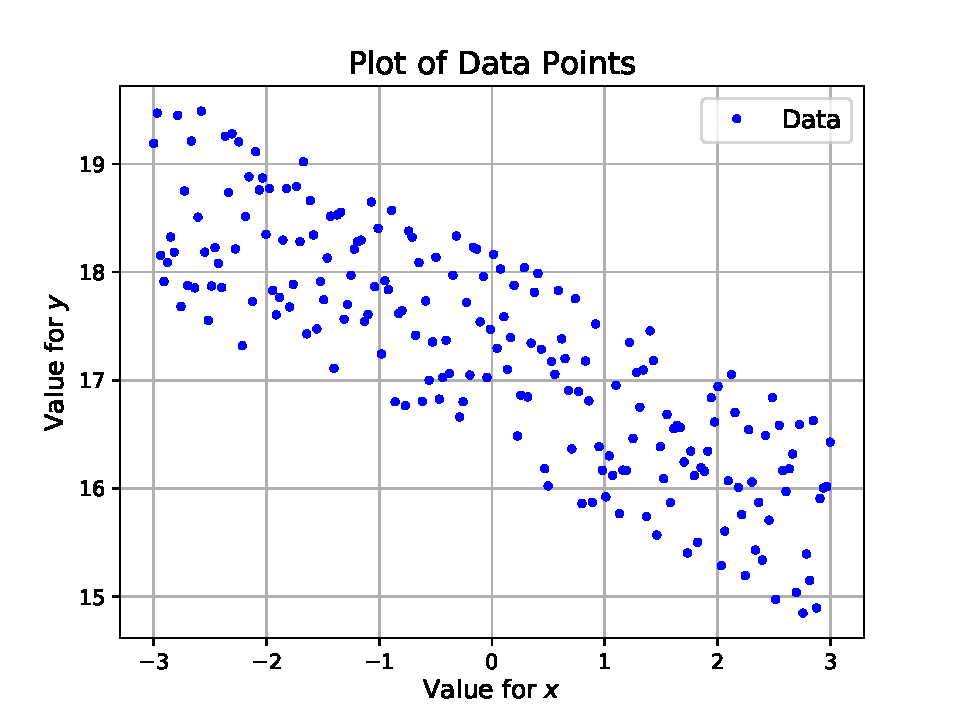
\includegraphics[width = 5in]{Data.pdf}
\caption{Plot of our given data coordinates}
\label{figLinearData}
\end{figure}

Firstly, we can make the assumption that our linear equation will have a negative gradient. There is a general slope in the data from top left to bottom right. Next, we can see  that our data passes through the $y$-axis within the boundary $16<y<19$. So we can assume that the intercept is positive. Combining these two observations will update our line of best fit to be
\begin{align*}
y = -mx + c
\end{align*}

Making these observations are simple yet very helpful in building up a good prior for our model, which we will do next.

\subsection{Choosing the Prior}\label{Choosing the Prior2}

We have our prior assumptions so now we can look into refining them. If we try and approximate the centre value at each end of the data cluster then we can think of these as two points. The points will be where our lines cross at $p_1 = (3,16)$, $p_2 = (-3,19)$. Then, if we were to plot a line through these two points, we will plot a linear line that will give us a visual idea of what the best fit line should look like. Plotting these graphs gives us the following.
\begin{figure}[H]
\centering
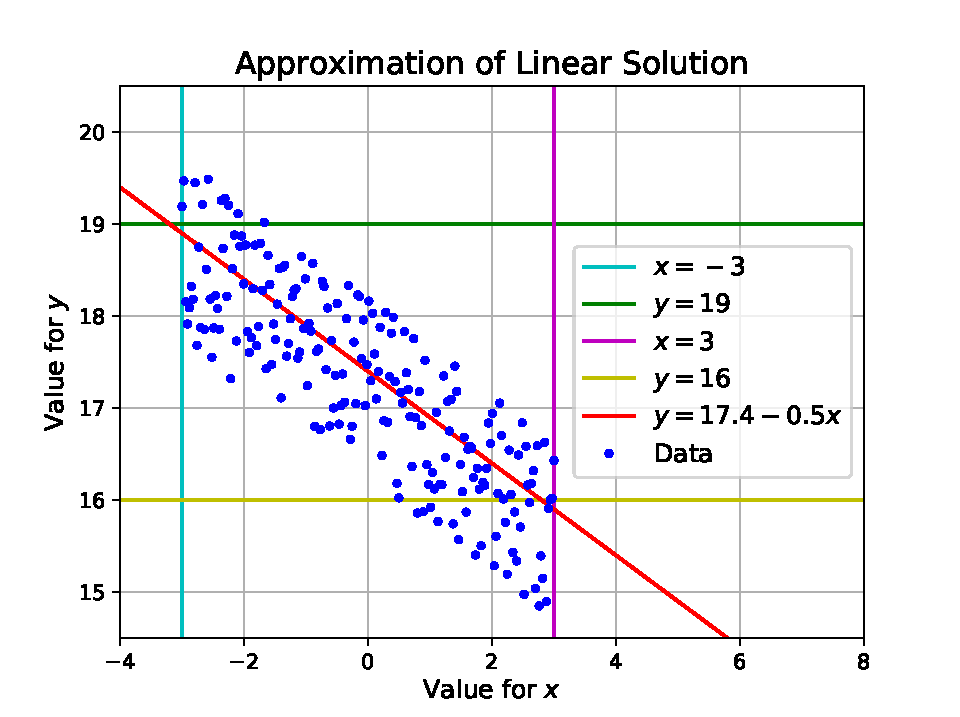
\includegraphics[width = 5in]{Approx.pdf}
\caption{Plot of approximate parameter values}
\label{figLinearDataLines}
\end{figure}

After studying the updated plot, we see that the intercept should be around $c\approx 17.4$ and that the gradient is around $m\approx -0.5$. It does not matter too much that our plot does not go through $p_1$ and $p_2$ because it is just to make the idea we have in our head more clear. To have some clarification mixed with some common sense. We will now be able to decide on our prior for our model but in the back of our minds we will, to some extent, expect to get values like this.

\subsubsection{The Intercept}\label{The Intercept}

We need to think about the best distribution to choose for the parameters we want to find. The distribution we are using here is the \textbf{Uniform} distribution as all possible values within the range are equally likely. The intercept, $c$, is a number that will lie between $16<y<19$. So the minimum is $16$ and the maximum is $19$. All of the data points around $x=0$ are \textbf{contained} within these values. I chose the prior for the intercept to be a uniform distribution. This is to say that any of the values between the lower and upper limits are equally probable
\begin{align*}
c \sim U(16, 19)
\end{align*}

\subsubsection{The Gradient}\label{The Gradient}

The gradient, $m$, is \textit{again} a number that will lie between $-1$ and $0$. Similarly, we have a lower and upper limit so we will also have our gradient prior as a uniform distribution
\begin{align*}
m \sim U(-1, 0)
\end{align*}

If we observe what these different gradients look like when compared to the data, it will help to see why we chose these values for our uniform priors. Our two comparisons are seen below
\begin{figure}[H]
\centering
\begin{subfigure}{0.5\linewidth}
  \centering
  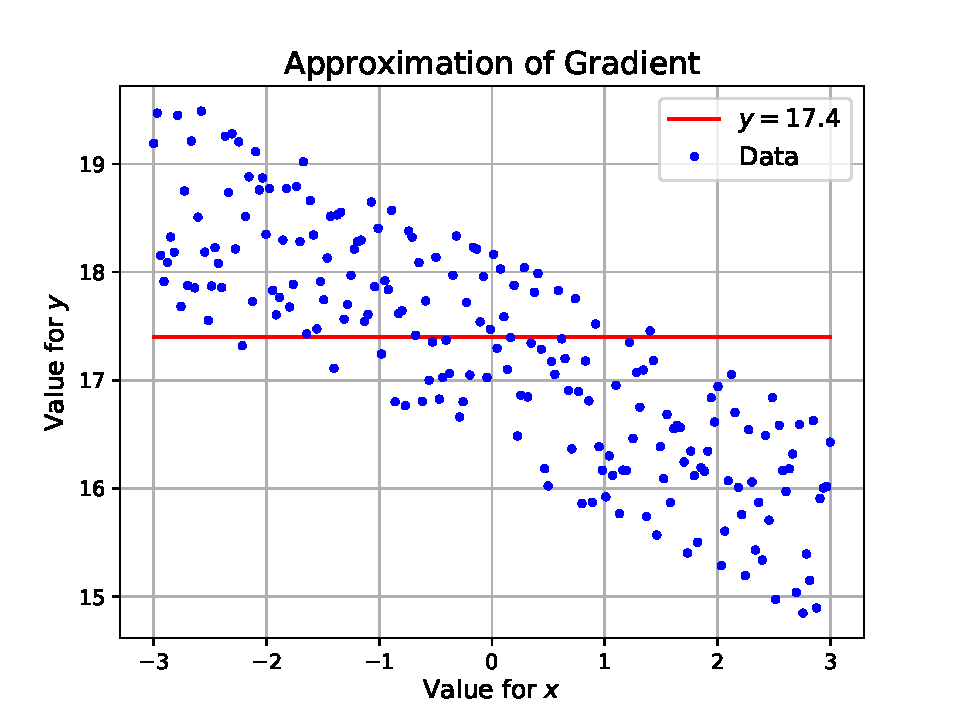
\includegraphics[width = 3in]{gradient0.pdf}
  \caption{Plot with $m = 0$}
  \label{fig:sub1}
\end{subfigure}%
\begin{subfigure}{0.5\linewidth}
  \centering
  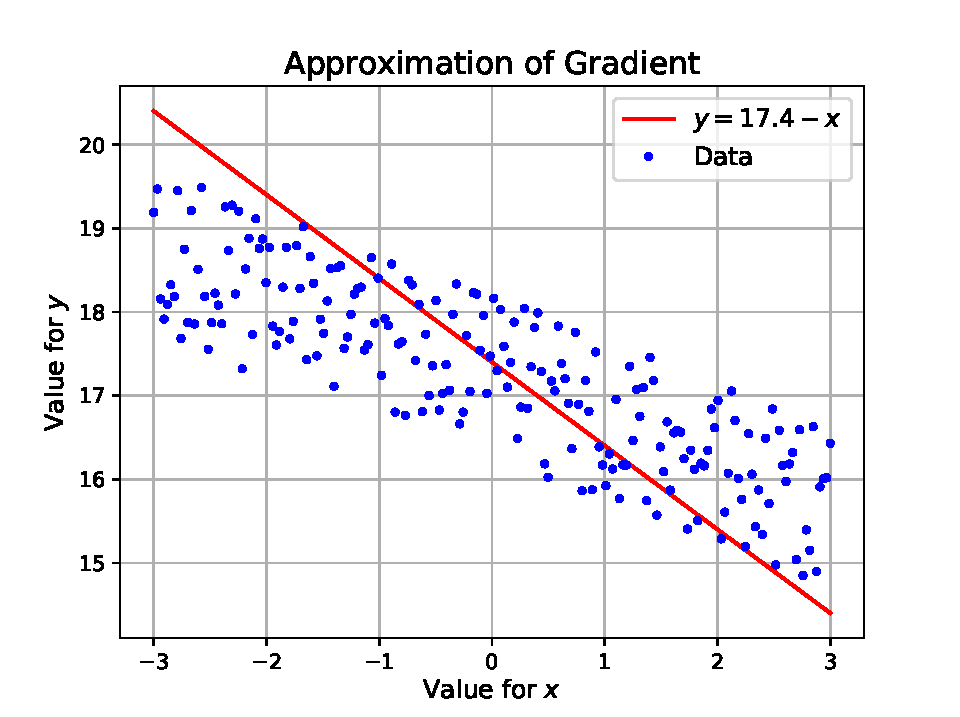
\includegraphics[width = 3in]{gradient1.pdf}
  \caption{Plot with $m = -1$}
  \label{fig:sub2}
\end{subfigure}
\caption{Comparison of data with different gradient values}
\label{fig:gradient}
\end{figure}

\subsection{Computing the Posterior}\label{Computing the Posterior2}

For this posterior we are not dealing with conjugate pairs. It does not matter because, as said in \S\ref{Choosing the Prior}, it is a way of producing an analytic solution. Using Python, it is a numerical approach instead.

\begin{lstlisting}[label={python code 1},caption={PyMC priors},language=Python]
	import pymc
	# Define variables with their prior distributions
	m = pymc.Uniform('m', -1, 0)
	c = pymc.Uniform('c', 16, 18)
\end{lstlisting}

First is to import the PyMC module so that we can incorporate the MCMC method. Next, we define variables $m$ and $c$ to be equal to uniform distributions using the modules built-in probability distributions functions. Using a uniform distribution means that all values in the range are equally probable. We set the variable along with the lower and upper limits. The function then calculates the pmf as
\begin{align*}
f(x\mid \mathrm{lower}, \mathrm{upper}) = \frac{1}{\mathrm{upper} - \mathrm{lower}}\quad\text{where}\quad\mathrm{lower}\leq x\leq\mathrm{upper}
\end{align*}

\ContinueLineNumber
\begin{lstlisting}[label={python code 2},caption={PyMC model},language=Python]
	# Define the form of the model
	@pymc.deterministic
	def y_model(xdata = xdata, c = c, m = m):
    	return c + m * xdata
\end{lstlisting}

We specify a model so that we can relate the parameters to the data. PyMC has three basic building blocks for Bayesian probability models. Here we are using the \texttt{Deterministic} object because the mean is a deterministic function of $m$, $c$ and $x$. We create \texttt{y\_model} by using the \texttt{deterministic} decorator and set it equal to a linear equation
\begin{lstlisting}[label={python code 3},caption={PyMC likelihood},language=Python]
	# Define likelihood
	y = pymc.Normal('y', mu = y_model, tau=1./(edata/2)**2,
	                observed = True, value = ydata)
\end{lstlisting}

Let us choose a normal distribution. This is written in the same way as the prior distributions. We set the variable along with $\mu$, the mean, and $\tau$ which is one over the standard deviation squared. For this example, the variable \texttt{edata} was just given the trivial value $1$ as there is no error associated with each individual point. The function then calculates the normal pmf as
\begin{align*}
f(x\mid\mu,\tau) = \sqrt{\frac{\tau}{2\pi}}\frac{\exp\left\{-\frac{\tau}{2}\left(\ln(x) - \mu\right)^2\right\}}{x}\quad\text{where}\quad\tau = \frac{1}{\sigma^2}
\end{align*}

\begin{lstlisting}[label={python code 4}, caption={PyMC MCMC implementation},language=Python]
	# package the full model in a dictionary
	model1 = dict(c = c, m = m, y_model = y_model, y = y)
	# run the basic MCMC
	S = pymc.MCMC(model1)
	S.sample(iter=100000, burn=50000)
\end{lstlisting}

This is where the computation of the posterior happens. It is where the power of PyMC lies. We store the four parameters into \texttt{model1} and then, using the command \texttt{pymc.MCMC.sample}, the \textbf{Markov Chain Monte Carlo} algorithm runs with 100,000 iterations and a burn-in of 50,000. This means that the first 50,000 iterations will be forgotten to ensure that MCMC collects values for the trace that converges to the normal (posterior) distribution.
\begin{lstlisting}[label={python code 5},caption={PyMC trace extraction},language=Python]
	# extract the traces and plot the results
	pymc_trace_unifo = [S.trace('c')[:],
    	                S.trace('m')[:]]
	plot_MCMC_results(xdata, ydata, pymc_trace_unifo)
	print() # Make a new line in the console window after S.sample
	print('c mean = {:.4f}'.format(pymc_trace_unifo[0].mean()))
	print('m mean = {:.4f}'.format(pymc_trace_unifo[1].mean()))
	print('c std = {:.4f}'.format(pymc_trace_unifo[0].std()))
	print('m std = {:.4f}'.format(pymc_trace_unifo[1].std()))
\end{lstlisting}

Finally, we define \texttt{pymc\_trace\_unifo} as the array that stores the trace of the parameters $c$, element \texttt{[0]}, and $m$, element \texttt{[1]}, using the \texttt{pymc.MCMC.trace} command. Line $20$ would give an error on its own. This is calling a function of functions defined earlier which will plot the parameter traces and the model. The traces are plotted into an \textbf{error ellipse} with a $68.3\%$ and $95.5\%$ credible interval.
\begin{figure}[H]
\centering
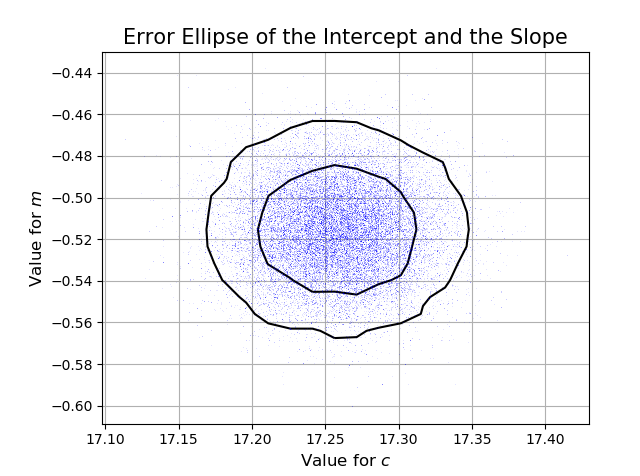
\includegraphics[width = 5in]{Ellipse.png}
\caption{Plot of the trace of $c$ and $m$}
\label{figEllipse}
\end{figure}

This gives us a beautiful cluster which represents the constrained relation between our two parameters. The region represents the two normal distributions (histograms) plotted together. We are able to take the two traces from our confidence ellipse and plot them individually. Then, we can calculate the mean and standard deviation and plot a normalised normal probability density function (pdf) over the histograms. The code below shows just how easy this is through PyMC in Python.
\begin{lstlisting}[label={python code 6},caption={Linear code pdf plotting snippet},language=Python]
	mu = pymc_trace_unifo[0].mean() # mean
	sigma = pymc_trace_unifo[0].std() # standard deviation
	x = pymc_trace_unifo[0]
	
	mu1 = pymc_trace_unifo[1].mean() # mean
	sigma1 = pymc_trace_unifo[1].std() # standard deviation
	x1 = pymc_trace_unifo[1]
\end{lstlisting}

From the histograms, and error ellipse, our final answer for our problem falls into what we expected in \S\ref{Choosing the Prior2}. This gives us further reassurance that what we have for our solution is a plausible solution to the problem.
\begin{figure}[H]
\centering
\begin{subfigure}{0.5\linewidth}
  \centering
  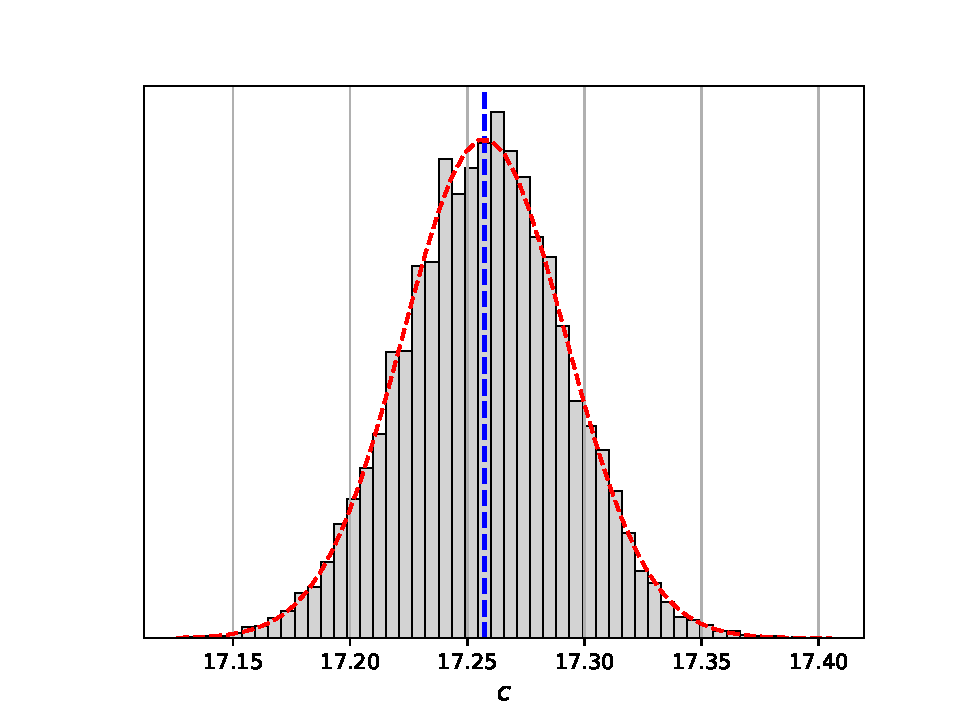
\includegraphics[width = 3in]{Histc.pdf}
  %\caption{Histogram of the intercept}
  \label{fig:subhist1}
\end{subfigure}%
\begin{subfigure}{0.5\linewidth}
  \centering
  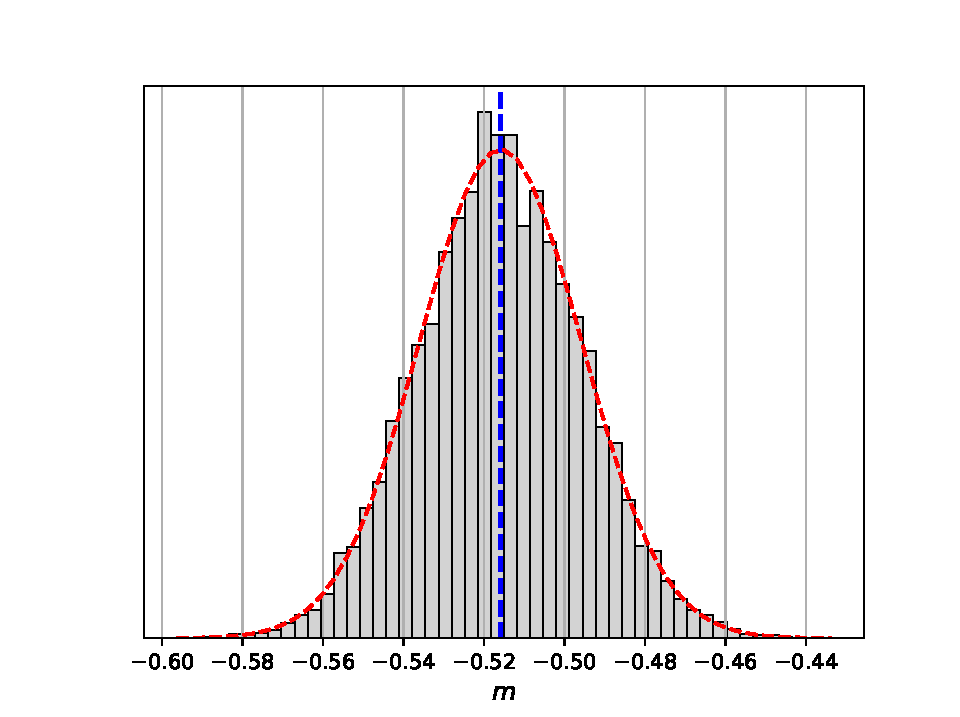
\includegraphics[width = 3in]{Histm.pdf}
  %\caption{Histogram of the gradient}
  \label{fig:subhist2}
\end{subfigure}
\caption{Histograms of the intercept and the gradient}
\label{fig:histograms1}
\end{figure}

Here I have given a similar representation of what the console output is when we run our code (line 21-25). It outputs the mean, represented by the dashed blue line, and standard deviation 
\small \begin{tcolorbox}[colback=black!5,colframe=black!40!black,title=\texttt{Terminal}]
\texttt{[--------------100\%--------------] 100000 of 100000 complete in 4.4 sec\\
c mean = 17.2573\\
m mean = -0.5159\\
c std = 0.0347\\
m std = 0.0202}
\end{tcolorbox}

Now we can then take these values and make one last plot over the data to see how our solution looks. The uncertainty region represents two standard deviations of the parameters.
\begin{figure}[H]
\centering
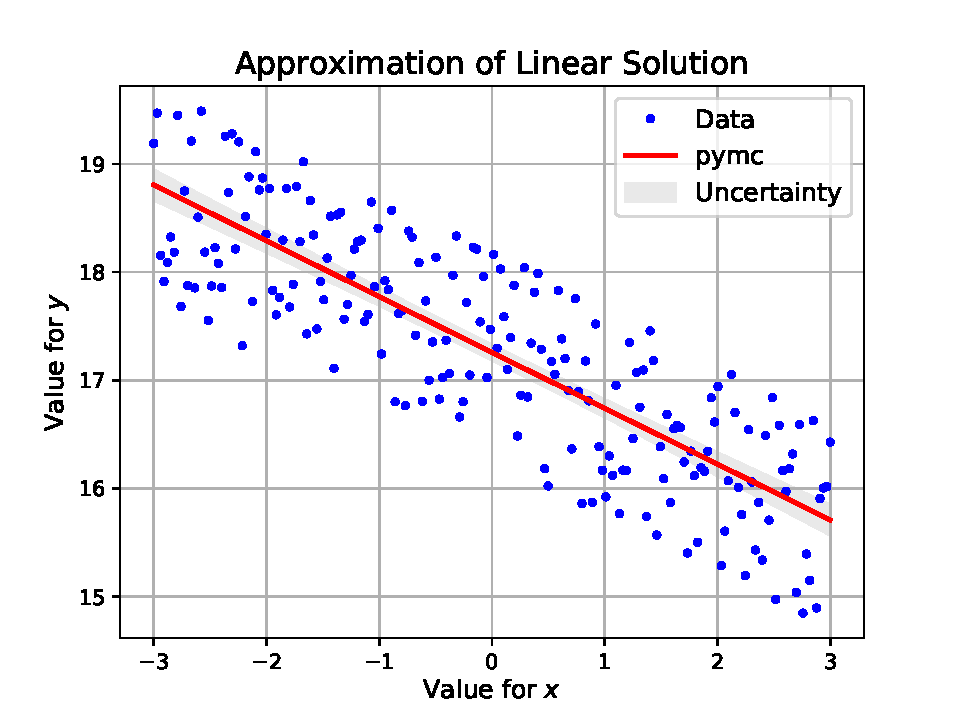
\includegraphics[width = 5in]{Finalgraph.pdf}
\caption{Plot of our linear solution}
\label{figFinalGraph1}
\end{figure}

\chapter{Global Warming}\label{Global Warming}

We now come to one of the main inspirations for my project. I am an environmentalist so I care about our blue planet and want to make sure that what I leave behind for my future generations is that caring for the environment is extremely important. And so, the topic of global warming is one that I really wanted to cover. Our linear regression example has given us the necessary basics we need to start looking into the ways that Python can be applied in real data analysis with data collected from around the world. We are going to investigate data related to the growth rate in atmospheric $\mathrm{CO_2}$ over the past years. From this we will then begin our data analysis methods to prove against big issues in our modern day society like the ridiculous belief that global warming is a myth.

\section{The Model}\label{The Model3}

We can access reliable data from repositories on the internet from the year 1960. The values of $\mathrm{CO_2}$ mole fraction increase (ppm) from $1^{\text{st}}$ January through $31^{\text{st}}$ December for years 1959 to 2017 is taken from the \textbf{National Oceanic and Atmospheric Association} (\textbf{NOAA}). The annual mean growth rate is the difference in concentration between the start and end of the year. $\mathrm{CO_2}$ mole fraction is measured at the Mauna Loa Observatory, Hawaii with an altitude of 3,400 meters. The process uses a $\mathrm{CO_2}$ analyser which transmits infrared light through the air that is measured by a sensitive infrared radiation detector. Carbon dioxide absorbs infrared radiation, which causes the earth surface temperature to increase, so the more $\mathrm{CO_2}$ in the air, the more absorption, the less light picked up by the detector. This measure in converted into the measure of $\mathrm{CO_2}$ mole fraction.

Mole fraction is defined as the number of $\mathrm{CO_2}$ molecules in a given of number of molecules of air e.g. if there are 256 parts per million (ppm) of $\mathrm{CO_2}$ this means that for every million molecules of air there are on average 256 $\mathrm{CO_2}$ molecules. The uncertainty is estimated using a Monte Carlo technique that computes 100 time series of global annual growth rates, each time using measurement records from a different sampling of sites from the NOAA ESRL cooperative air sampling network.

(For more information see \cite{4})

Coding this in Python to read in the data, that can be downloaded from the NOAA website, and then plotting the data gives the following figure
\begin{figure}[H]
\centering
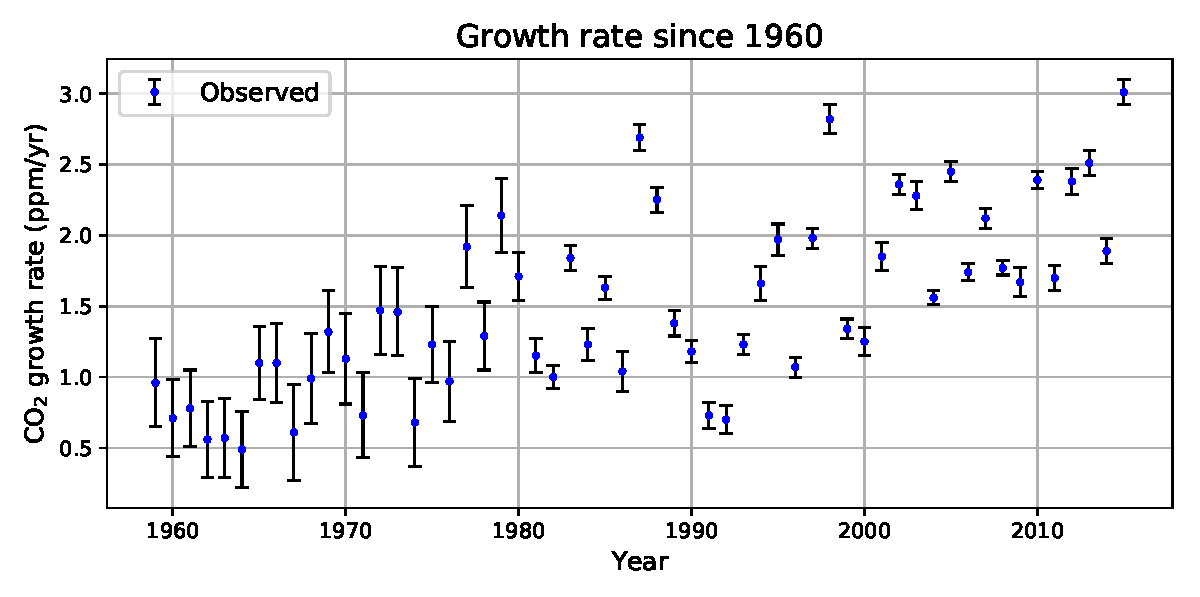
\includegraphics[width = 6in]{FullDataPlot.pdf}
\caption{Plot of our data coordinates}
\label{figFullDataPlot}
\end{figure}

We see the measurements with their uncertainty. We can now start investigating the data, to give evidence that the level of $\mathrm{CO_2}$ in the atmosphere is rising. This can be shown with a linear regression. By taking the error associated with each observation, we can calculate a best fit line and present the results. As we covered the approach in such detail with \S\ref{Linear Example}, we can cover the process more quickly.

\subsection{Computing the Posterior}\label{Computing the Posterior3}

This code is slightly different to Listing \ref{python code 1}-\ref{python code 5} but still achieves the similar results.
\StartLineAt1
\begin{lstlisting}[label={python code 7},caption={Climate change code snippet},language=Python]
	import pymc
	def model(x, y): 
    	slope = pymc.Normal('slope', 0.1, 1.)
    	intercept = pymc.Normal('intercept', -50., 10.)
    	@pymc.deterministic
    	def linear(x=x, slope=slope, intercept=intercept):
        	return x * slope + intercept
    	f = pymc.Normal('f', mu=linear, tau=1.0/y_error,
    	                value=y, observed=True)
    	return locals()
	MDL = pymc.MCMC(model(x,y))
	MDL.sample(5e5, 5e4, 100) # iter=500,000, burn=50,000, thin=100
	pymc_trace_unifo = [MDL.trace('slope')[:],
                      MDL.trace'`intercept')[:]]

	print('slope = {0:.3f}, intercept = {1:.2f}'.format(
	                                     pymc_trace_unifo[0].mean(),
	                                     pymc_trace_unifo[1].mean())
\end{lstlisting}

Lines 3-4 define the prior distributions. Lines 5-8 define the likelihood. This is good because a normal prior is a conjugate prior to the normal distribution, giving us a normal distribution posterior. Lines 10-13 use MCMC but with the addition of a thinning value. This means that after the first 50,000 iterations, MCMC will save every 100th iteration giving a trace of 4,500 values rather than 450,000 (default thin=1) for the two parameters. 

Then, using the same approach as in Listing \ref{python code 6}, I can use the trace, mean and standard deviation to plot the posterior distribution over the histograms for the two parameters.
\begin{figure}[H]
\centering
\begin{subfigure}{0.5\linewidth}
  \centering
  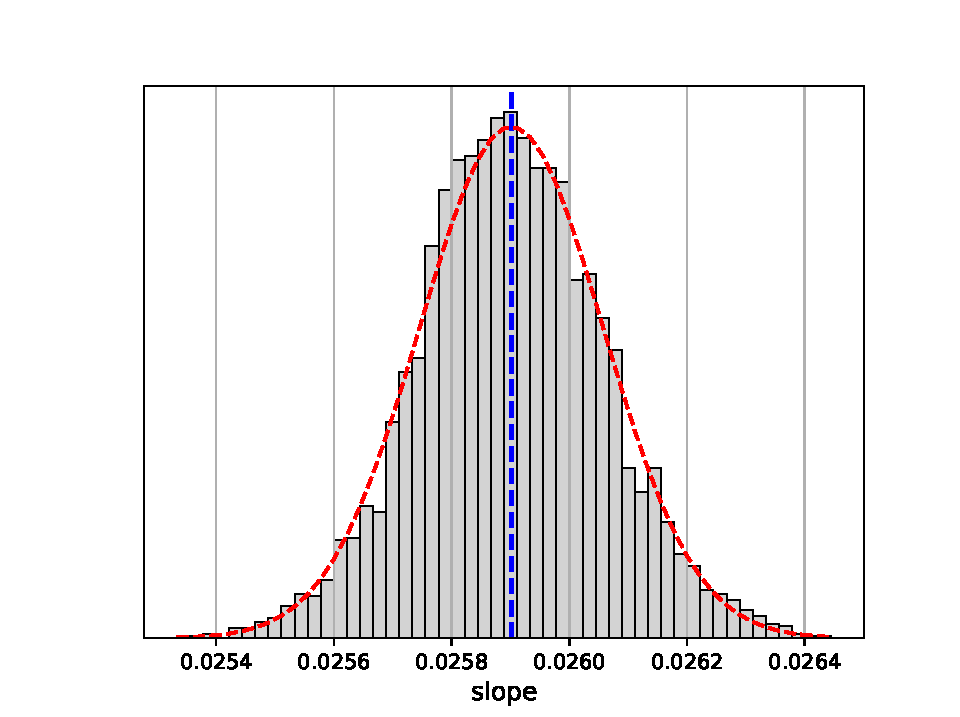
\includegraphics[width = 3in]{slope.pdf}
  %\caption{Histogram of the intercept}
  \label{fig:subslope}
\end{subfigure}%
\begin{subfigure}{0.5\linewidth}
  \centering
  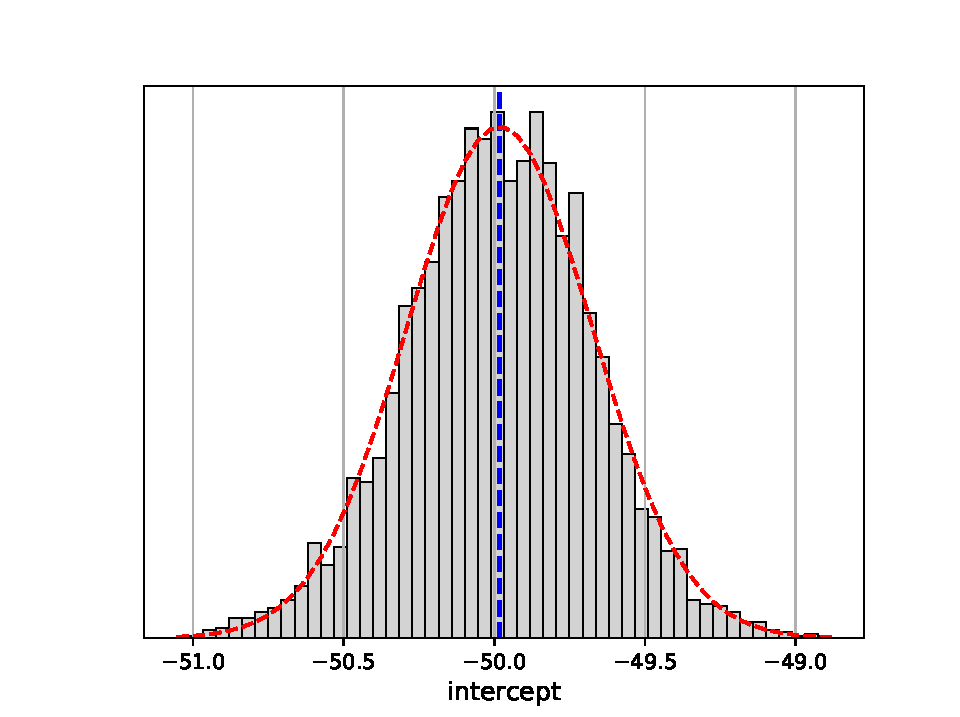
\includegraphics[width = 3in]{intercept.pdf}
  %\caption{Histogram of the gradient}
  \label{fig:subintercept}
\end{subfigure}
\caption{Histograms of the slope and intercept}
\label{fig:histograms2}
\end{figure}

The console output is similar as well but with a longer run time with more iterations of MCMC.
\small \begin{tcolorbox}[colback=black!5,colframe=black!40!black,title=\texttt{Terminal}]
\texttt{[---------------100\%---------------] 500000 of 500000 complete in 17 sec\\
slope = 0.026, intercept = -49.98}
\end{tcolorbox}

Finally, we can plot our linear regression over our data.
\begin{figure}[H]
\centering
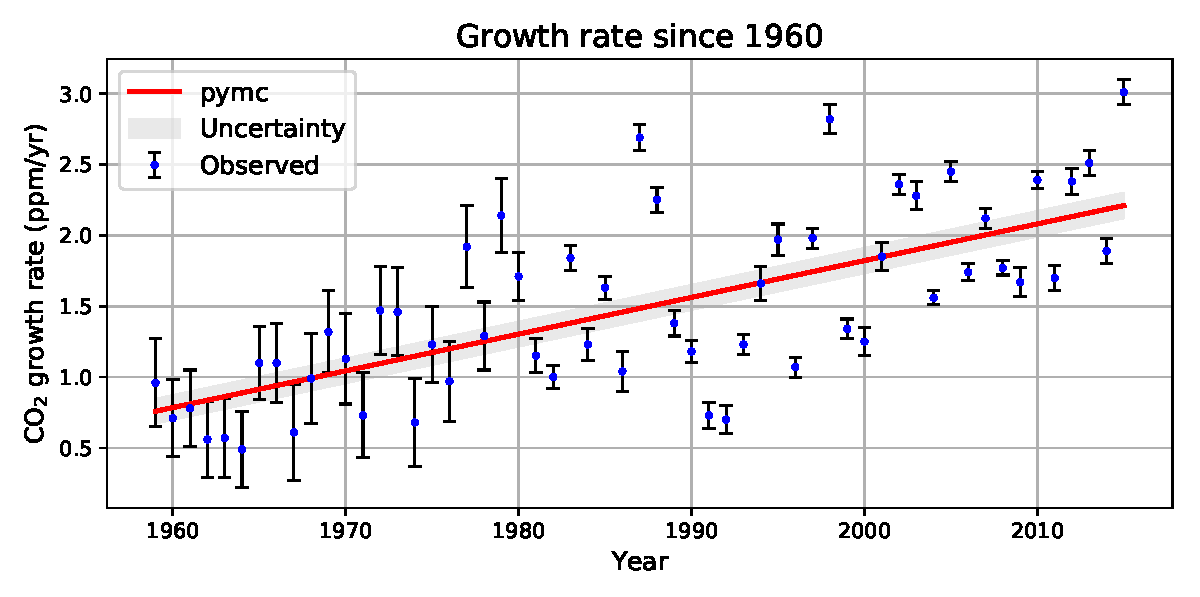
\includegraphics[width = 6in]{FinalClimate.pdf}
\caption{Plot of our linear regression}
\label{figFinalGraph2}
\end{figure}

There is a linear regression related to the increase in atmospheric $\mathrm{CO_2}$ levels and, with a positive gradient, this level is increasing which should be all the evidence we need to start putting green solutions in place to prevent climate change as much as possible. If we are more than lucky, the damage done can be reverted. Many people will only listen when the solution does not change the lifestyle that they have become so used to but this is where a deeper problem lies.

Only through changing the way we live our everyday lives will we be able to prevent any further damage to our fragile world, our beautiful blue planet and all the life that exists on it. We as a species need to accept the fact that things cannot be the way they have been for the past 70 years. It is not just our duty as the ones responsible for the damage to change the way we live for a cleaner alternative but our reason for being. 

This is the one place that formed billions of years ago in the perfect spot of us to evolve into what we are today. We cannot lose something this precious, something so irreplaceable, because we are too foolish to heed the warnings of science. If it has brought us this far, it can take us further still.

We have reached the final advance of this thesis, with a topic that I find very interesting! Using observations of supernova redshift, we can estimate the fraction of dark energy and dark matter in the universe. But how? Let's see.

(See \cite{1} for more detail in \S\ref{Global Warming})

\chapter{Dark Energy, Dark Matter and Hubble's Parameter}\label{Dark Energy}

This topic will take us beyond our planet and out into the stars. First, we have the theory that
\begin{align}\label{curvature}
\Omega_\Lambda + \Omega_M + \Omega_{\text{curvature}} &= 1\notag \\
\Rightarrow\quad\Omega_{\text{curvature}} &= 1 - \Omega_\Lambda - \Omega_M
\end{align}

where $\Omega_\Lambda$ is the fraction of dark energy, $\Omega_M$ is the fraction of dark matter. These parameters relate to the expansion of the universe. Dark energy causes expansion of the universe and dark matter causes compression of the universe. With the observation of redshift from distant supernovae, this suggests that there is more dark energy in the universe than dark matter. Otherwise we would observe the much more rare blueshift. The task to find out if our findings match this hypothesis.

Our data is observations of many supernovae that have been grouped together into $31$ \texttt{bins}. With the value of redshift for each \texttt{bin}, we can calculate the values of the \textit{distance modulus}, $\mu_b$, using the following
\begin{align}\label{distance modulus}
\mu_b(z) = 25 + 5\log_{10}(D_L(z_b))\,\,\text{for redshift}\,\,z_b
\end{align}

where the variable $D_L(z)$ is given by
\begin{align*}
D_L(z_b) = \frac{2998}{h}(1+z_b)\int_0^{z_b}\left(\frac{1}{\sqrt{\Omega_\Lambda + \Omega_M(1+x)^3 + (1 - \Omega_\Lambda - \Omega_M)(1+x)^2}}\right)\,\mathrm{d}x
\end{align*}

This complicated integral contains three unknown parameters. The first two in equation (\ref{curvature}) and Hubble's parameter
\begin{align*}
h = \frac{H_0}{100}\,\,\text{where $H_0$ is Hubble's constant}
\end{align*}

It roughly quantifies how quickly the Universe is expanding at present. Hubble's constant has unit of measurement kilometer per second per megaparsec or $\mathrm{kms}^{-1}\mathrm{Mpc}^{-1}$. This is confusing but, if we consider the dimensions, we have
\begin{align*}
H_0 = \frac{L}{T}\cdot L^{-1} = T^{-1}
\end{align*}

So Hubble's constant has unit $\mathrm{s}^{-1}$. But, the reason this isn't the preferred unit is because if we consider Hubble's constant measured by Planck, 67$\mathrm{kms}^{-1}\mathrm{Mpc}^{-1}$, and convert to the unit per second this gives $2.2\times10^{-18}\mathrm{s}^{-1}$. This is more difficult to remember than 67 so it is used for convenience.

All three of these parameters have joint constraints to each other. If $h$ changes then it changes the other two parameters and vice versa. We need to model equation (\ref{distance modulus}) in Python with this in mind.

\section{The Model}\label{The Model4}

We have the following data from Table \ref{tab:mub} (the mean values) and the \textit{``covariance matrix''} which quantifies the error in the data. This is a symmetric matrix that has dimension 31, corresponding to the number of supernovae \texttt{bins}. The diagonal of the matrix gives $\sigma^2$ for each measurement in Table \ref{tab:mub}. Taking the square root will give us the standard deviation.

The task at hand is to fit all these observations using only three parameters $\Omega_\Lambda$, $\Omega_M$ and $h$. Our first step is to plot $\mu_b$ against $z_b$ along with the standard diveation associated with each point. In Python, we can writing the digonal of the matrix as a single array, multiply each value by $10^{-6}$, square root each value and store the variable \texttt{edata} as this array. So, the plot of the observations is the following 

(The table, covariance matrix and information see \cite{5})
\begin{figure}[H]
\centering
\begin{subfigure}{0.5\linewidth}
  \centering
  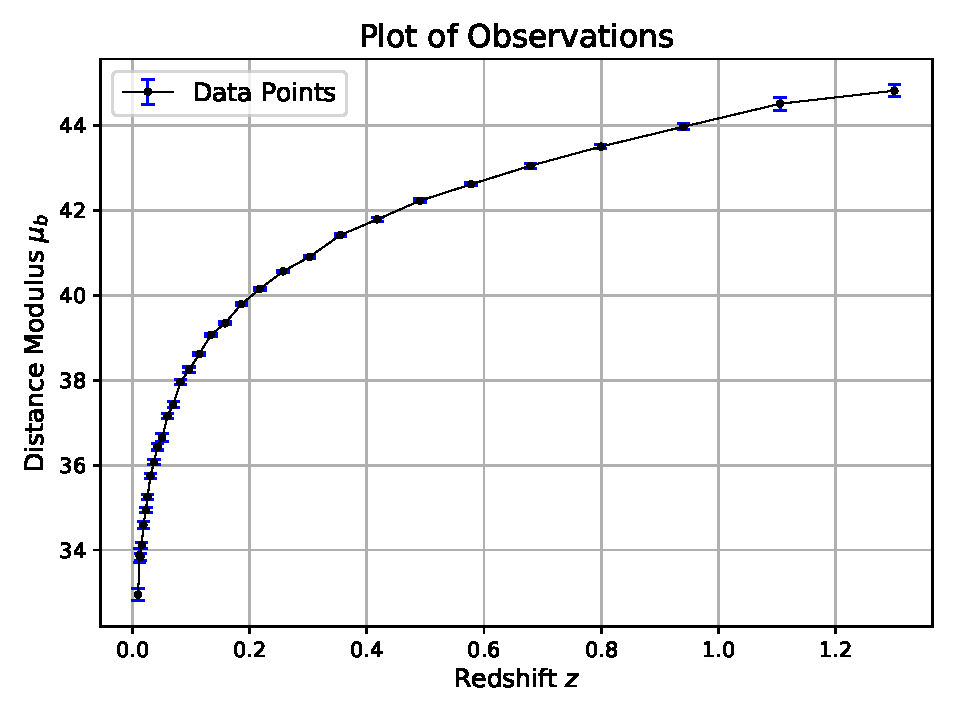
\includegraphics[width = 3in]{SupernovaeDataCurve.pdf}
  \caption{Plot of supernovae observations}
  \label{fig:curve}
\end{subfigure}%
\begin{subfigure}{0.5\linewidth}
  \centering
  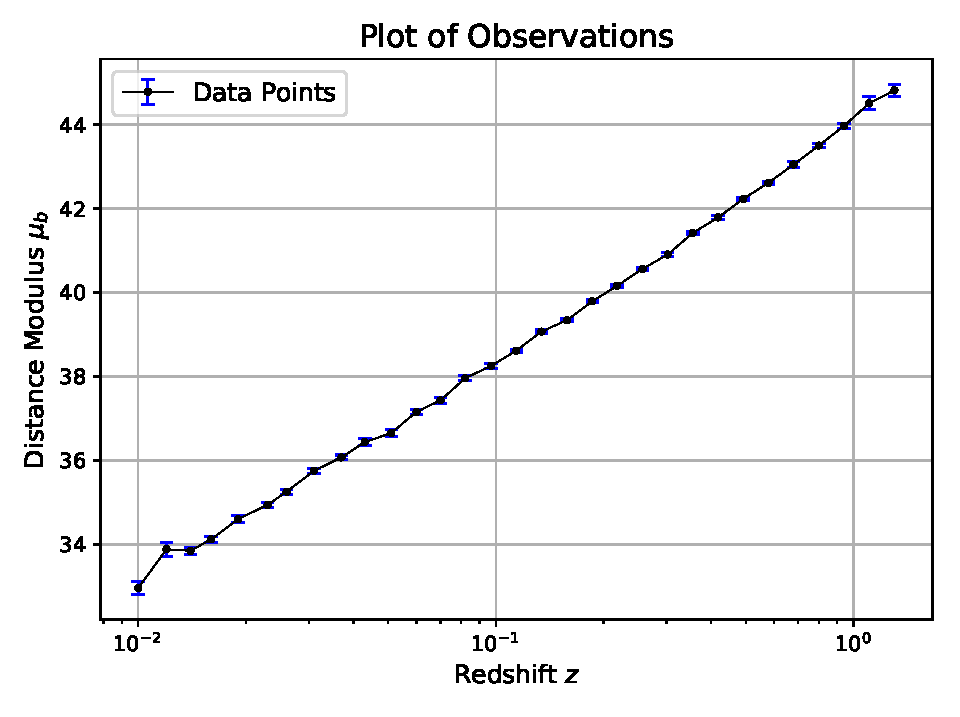
\includegraphics[width = 3in]{SupernovaeDataLog.pdf}
  \caption{Log plot of \ref{fig:curve}}
  \label{fig:log}
\end{subfigure}
\caption{Comparison of data with different redshift scale}
\label{fig:SupernoveData}
\end{figure}

Our plan from here is different from our previous chapters. We want to estimate the parameters that fit the data. This task does not require us to try and fit a line through the data, but to produce distributions of the parameters and see what they come out to be.
\pagebreak
\subsection{Computing the Posterior}\label{Computing the Posterior4}

Just as before, we observe some Python code because there are important changes being made
\StartLineAt1
\begin{lstlisting}[label={python code 8},caption={Supernovae code snippet},language=Python]
	# Data from Planck Mission March 21, 2013
	Omega_Lambda = pymc.Normal('Omega_Lambda', 0.65, 100) #
	Omega_M = pymc.Normal('Omega_M', 0.25, 100) #
	h = pymc.Normal('h', 0.65, 100)
	@pymc.deterministic
	def y_model(xdata=xdata, Omega_Lambda=Omega_Lambda,
	            Omega_M=Omega_M, h=h):
    	mu_b = [0] * len(xdata)
    	if Omega_M<0.05:
        	Omega_M=0.05
    	if Omega_M>0.45:
        	Omega_M=0.45
    	if Omega_Lambda<0.45:
        	Omega_Lambda=0.45
    	if Omega_Lambda>0.85:
        	Omega_Lambda=0.85
    	def Formula(x):
        	root= sqrt(Omega_Lambda + Omega_M*(1 + x)**3 +
        	           (1 - Omega_Lambda - Omega_M)*(1 + x)**2)
        	result = 1/root                
        	return result
    	for i in range(len(xdata)):
        	z = xdata[i]
        	D_L = ((2998/h)*(1 + z))*quad(Formula, 0, z)[0]
        	mu_b[i] = 25 + 5*log10(abs(D_L))
    	return mu_b
	T = np.linalg.inv(my_cov) # tau = precision matrix = inverse of covariance matrix
	y = pymc.MvNormal('y', mu=y_model, tau=T,
	                  observed=True, value=ydata)
	# package the full model in a dictionary
	model1 = dict(h=h, Omega_Lambda=Omega_Lambda,
	              Omega_M=Omega_M, y=y)
	# run the basic MCMC:
	S = pymc.MCMC(model1)
	S.sample(iter=100000, burn=80000)
	# extract the traces and plot the results
	pymc_trace_unifo = [S.trace('h')[:],
                    	S.trace('Omega_Lambda')[:],
                    	S.trace('Omega_M')[:]]
\end{lstlisting}

Lines 1-3 are normal priors. By searching the internet, it can be found that $\Omega_M \approx 26.8\%$ of the universe is dark matter, $\Omega_\Lambda \approx 68,3\%$ is dark energy and Hubble's constant $H_0 \approx 73\mathrm{kms}^{-1}\mathrm{Mpc}^{-1}$. Rather than using a uniform prior saying that all values from 0 to 1 are equally likely we will give them a normal distribution set around a value that reflects what has been proposed by others and seeing what the data gives. $\tau = 100$ means our standard deviation is $\sigma = 0.1$ e.g. for $\Omega_M = 0.25 \pm 0.1$ or $25\%\pm10\%$. \texttt{y\_model} is no longer a simple linear equation but instead the complicated equation \ref{distance modulus}. Line 8 creates a list of 31 zeros to be over 9-16 control the parameter values being passed to the integrand so that we do not take the square root of a negative number or divide by 0 at line 18 and 20. It also acts to have the spread set at a maximum and minimum of $2\sigma$ to help the convergence of MCMC look tighter in our error ellipse.

Using a value from each parameter, lines 22-26 loop through the 31 different values for $D_L(z)$ and $\mu_b(z)$ respectively and stores them as the array \texttt{mu\_b}. Lines 27 and 28 calculate the inverse of the covariance matrix and define the likelihood as the multivariate normal. Since we are dealing with 3 normally distributed parameters, the multivariate normal is a generalisation of normal distribution (univariate). Our loop will then be repeated, in this example, 100,000 times by MCMC (using the last 20,000 for our plot). Because of the amount of dimensions we are dealing with, this makes the computations much longer. This run of MCMC took 491.8 seconds. But this manages to give us pretty clear graphs displayed below
\begin{figure}[H]
\centering
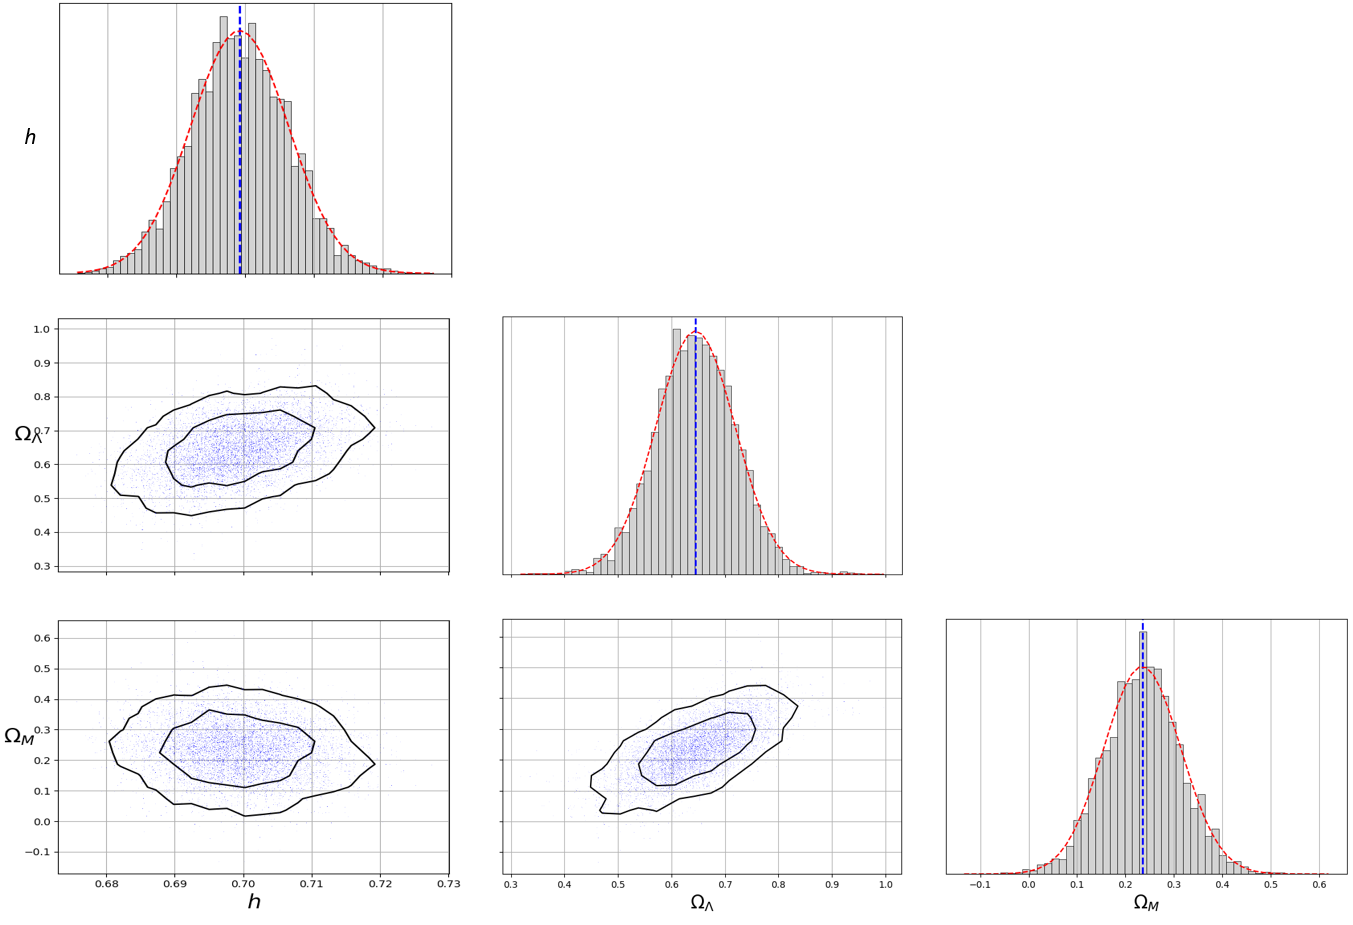
\includegraphics[width = 6in]{triangle.png}
\caption{Constraint relation between $h$, $\Omega_M$ and $\Omega_\Lambda$}
\label{figConstraint}
\end{figure}

This is an amazing result! The three error ellipses show why the use of a multivariate normal is required. If we view the column for parameter $h$ we see the normal distribution constrained by the normal distribution of $\Omega_M$ and $\Omega_\Lambda$. The same is for the $\Omega_M$ row. It gives us a visual understanding for the use of a multivariate normal function. What is even more exciting is what these figures suggest for our universe. 
\pagebreak

Extracting the values for the mean and standard deviation used in figure \ref{figConstraint}, we find that
\begin{align*}
\Omega_M = 23.47\% \pm 7.69\%,\quad\Omega_\Lambda = 64.49\% \pm 7.42\%,\\
H_0 = \frac{h}{100} = 69.92\mathrm{kms}^{-1}\mathrm{Mpc}^{-1} \pm 0.71\mathrm{kms}^{-1}\mathrm{Mpc}^{-1}
\end{align*}

We have been able to estimate a value of our three parameters. I for one think this is truly incredible that anyone can have Python on their home computer and these are the extraordinary things we can do. It truly is a wonderful time to be alive.

This goes to prove our hypothesis too. The universe was observed to be expanding by Edwin Hubble himself, but the question of just how fast remained. It was considered that the force of gravity would contribute to a retardation of the expansion. When astrophysicists set out to calculate the deceleration it was found that the expansion was not slowing down at all. It was accelerating. This means that there was something that was counteracting gravity given the name dark energy. Our findings show that $\Omega_M < \Omega_\Lambda$. So this would indicate what was observed is true. The universe expansion is accelerating because there is more dark energy than dark matter.

\chapter{Conclusion}

This is where I wanted to take some time to conclude my thesis on Python for mathematical applications. I have been able to accomplish a lot during my time studying Python. From dealing with a linear regression to much more complicated tasks, I have been able to show the tricks of the data science trade and it has only been one semester. There is still much to learn about the most advanced uses of Python.

I have been able to cover the main goals I set myself in this thesis. To give details into how the core part of PyMC works with the MCMC algorithm, to show how Python implements statistical mathematics like pdf through PyMC with ease and to present real life examples where Python can be used for official data analysis.

I also wanted to discuss what might have been done differently if more time was provided. I would have liked to include a chapter of what I learned in first year that I covered in my first semester presentation \textit{Solving ODE's with Python}. There was an example in which a data set was generated from a quadratic equation but time ran short to include this after the chapter linear regression.

Having more time would have allowed the figure of chapter 5 to be slightly improved. One improvement would be to add more plots, like a comparison of the posterior with the prior in the three parameter histograms. It would also allow me to explore the examples covered even further. To expand on chapter 5 by possibly including more parameters so that we can refine each parameter even more. 

But, to conclude my overall inspirations, I thoroughly believe that Python is a truly extraordinary tool. It has hundreds of applications that I have only scratched the surface upon. Not only does it help make the numerical analysis so much easier, it will improve my desirability for future employers. After realising my enthusiasm for computer programming, I will continue to learn Python so that I can pursue a career in computer science.

Being able to undergo this project has kick started a passion that I never thought could be possible. To know a computer language and have a degree in mathematics will, hopefully, open all the doors that will lead me onto my future dream job.

\chapter*{Acknowledgements}
\thispagestyle{plain}

I would like to take this opportunity to thank the people in my life who have given me the support I needed to make it this far in my academic lifetime, and the faith they will continue to bestow upon me to succeed in the future. 

Thank you to my mother, Christina Turner, and my father, Leonard Turner, for always helping me to achieve the best that I can be. You have always been there to give me guidance through the hardest times in life, and I will always be grateful. Thank you mother for giving me what little you had just to make me happy as a boy, and to my father for teaching me the important lessons of life and how to make the most out of what you have. The best way that can begin to repay you both for giving me the best start in life is to do my very best to make you proud.

Thank you to my auntie, Diane Greening, for your constant care and being the person in my life who introduced me to the world of science. Going to scientific talks and visiting observatories around the country will always be happy memories of mine. Taking an interest in science is what began my journey of discovery into my natural ability with mathematics. This might not have ever happened if without your influence.

Thank you to my partner, Rebecca Baker. No matter how stressed I might be and how distant I might become, your warming embrace and endless love will always bring me back. Regardless how difficult I might be to deal with at my worst, you stayed by my side, so that I can get through it all to be at my best. Thank you for sticking by me.

Thank you to my sister, Kerri-Marie Turner, for always being able to make me laugh when I was feeling down. You showed me how I can live life seeing the brighter side of life. That good things will come to those who deserve it.

And finally, thank you to my Grandmother, Kathleen Greening. The times I would stay with you while I was young were that sweetest of times. Playing with friends and riding in my old pedal kart. Thank you for taking care of me from my years at primary school to my years at university.

\bibliographystyle{acm}
\bibliography{Ref}
\pagebreak

\appendix
\chapter{Tables}

\begin{table}[H]
  \centering
  \caption{Binned distance modulus fitted to the JLA sample.}
  \label{tab:mub}
    \begin{tabular}{*{2}{rr|}rr}
    \hline
    \hline
    $z_b$ & $\mu_b$ &$z_b$ & $\mu_b$ &$z_b$ & $\mu_b$ \\
\hline
0.010 & 32.9538  & 0.051 &  36.6511 &  0.257 &  40.5649\\
0.012 & 33.8790  & 0.060 &  37.1580 &  0.302 &  40.9052\\ 
0.014 & 33.8421  & 0.070 &  37.4301 &  0.355 &  41.4214\\
0.016 & 34.1185  & 0.082 &  37.9566 &  0.418 &  41.7909\\
0.019 & 34.5934  & 0.097 &  38.2532 &  0.491 &  42.2314\\
0.023 & 34.9390  & 0.114 &  38.6128 &  0.578 &  42.6170\\
0.026 & 35.2520  & 0.134 &  39.0678 &  0.679 &  43.0527\\
0.031 & 35.7485  & 0.158 &  39.3414 &  0.799 &  43.5041\\
0.037 & 36.0697  & 0.186 &  39.7921 &  0.940 &  43.9725\\
0.043 & 36.4345  & 0.218 &  40.1565 &  1.105 &  44.5140\\
&&&&                                        1.300 &44.8218\\
    \hline
  \end{tabular}
\end{table}

\end{document}
